
\graphicspath{ {0chapterTheory/image/} }
\chapter{Theoretical Background}
\section{Digital Topology and Self-Duality}
\paragraph{}
A self-dual operator processes the image contents regardless its contrast \cite{Geraud.15.ismm}. In general, operators that are not self-dual do not treat bright objects over dark background and dark objects over bright background similarly which is often an undesirable feature. It is most important when no assumption about the contrast between object and background can be made. As any part of the images could be the subject, we want an operation which behavior the same way regardless the contrast between the subject and its background to obtain a unique representation.  
\begin{figure}

	\begin{subfigure}{0.3\textwidth}
	 	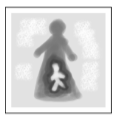
\includegraphics{im1.png} \caption{}\label{fig:gray} \end{subfigure}
	\begin{subfigure}{0.3\textwidth}
		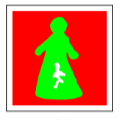
\includegraphics{im2.png} \caption{}\label{fig:mother} \end{subfigure}
	\begin{subfigure}{0.3\textwidth}
		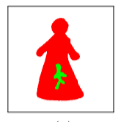
\includegraphics{im3.png} \caption{}\label{fig:baby} \end{subfigure}
	\centering
	\caption[Example of \textit{subjects}] {From the original gray level image \ref{fig:gray}, the subject can be either the mother \ref{fig:mother} (dark over bright) or the baby \ref{fig:baby} (bright over dark) }
	\label{fig:motheAndBaby}
\end{figure}

\paragraph{}
As we can seen in \ref{fig:motheAndBaby}, where green and red respectively represent the background and foreground. From the grayscale image \ref{fig:gray} If we focus in the mother, then the outer zone will be the background as in \ref{fig:mother}. Furthermore, we can chose the baby as the subject and therefore, the woman will become the background \ref{fig:baby}.	
\paragraph{}
For a image defined in the regular cubical grid, the digital topology must be describe by a "Jordan pair" of connectivity $(c_\alpha,c_\beta)$ \cite{Kong:1989:DTI:71397.71400}. One connectivity is used for the object and the other one for the background. This arbitrary choice affect the topology and self-dual operation must use different connectivity for the complementation to work in the same way.




\section{Well-composed Images}
\paragraph{}
As defined in \cite{Latecki95}, a 2D set S is weakly well-composed if any 8-component of S is a 4 component. S is well-composed if both S and its complement $\bar{C}$ are weakly well-composed. It can also be defined using the notion of "critical configurations" which are 
\includegraphics{confi1.jpg} and 
\includegraphics{confi2.jpg} : S is weakly well-composed if these configuration do not appear.
\paragraph{}
The notion of well-composednessed has also been extended to gray-level images. A gray-level image $\mu$ is well-composed if any set $[\mu \geq \lambda ]$ is well-composed. The extended version of "critical configuration" is that every block 
\begin{tabular}{|c|c|}
\hline 
a & d \\ 
\hline 
c & b \\ 
\hline 
\end{tabular} 
must verify interval(a,b) $\cap$ interval(c,d) $\neq \varnothing$ , where interval(a,b) = [min(a,b),max(a,b)].
\paragraph{}
An image is not a priori well-composed. There are 2 approach to get a well-composed image from the original image \cite{Geraud.15.ismm} by changing it pixel value (with possibility of alter the image's topology) or by a well-composed interpolation.



\section{Connected filter}
Motivated by families of filters by reconstruction, the notion of filter by reconstruction is introduced in \cite{Salembier95flatzones} \cite{Serra1993}. It work by simplifier the topographic map of images. The most important feature of this type of operator is preservation of contours \cite{Salembier2009}: they does not create new contours nor shift them.
\subsection{Morphological Tree-Based Image Representation}
One strategy to define connected operators replies on a hierarchical region-based representation of the input image, in another word, a tree. The filtering step is done by pruning that tree and the output image is compute by reconstructing the pruned tree.  Tree of shapes is a contrast-invariant image representation which is defined in \cite{Monasse.2000}.
\paragraph{} \textbf{A Couple of Dual Trees}: given an image $\mu $ in nD: $\mathbb{Z}^{n} \rightarrow \mathbb{Z} $, the lower cuts of $\mu$ are defined by 
	$[\mu < \lambda] =\lbrace x \in X \vert \mu (x) < \lambda \rbrace $. The set of all connected components of all these cuts is $ \mathcal{T}_< (\mu) =\lbrace \Gamma \in \mathcal{C}\mathcal{C}([\mu < \lambda]) \rbrace $ (with $\mathbb{C}\mathbb{C}$ denote the operator that takes a set and gives its set of connected component. As these sets verify $\forall \Gamma$ and $\Gamma ' \neq \lambda$, $\Gamma \subset \Gamma ' $ or $\Gamma \cap \Gamma '= \emptyset$, they can be arranged into a tree, called the \textit{min-tree} (because it if form using lower cuts, and the leaves will be minimum of image). We can also consider the upper cuts $[\mu \geq \lambda] =\lbrace x \in X \vert \mu (x) \geq \lambda \rbrace $, the element of $ \mathcal{T}_\geq (\mu) =\lbrace \Gamma \in \mathcal{C}\mathcal{C}([\mu \geq \lambda]) \rbrace $ will be arranged in to the \textit{max-tree}. The \textit{max-tree} and \textit{min-tree} are dual by complementation, the max-tree of $\mu$ is the min-tree of $ \mu$, therefore operations define on them are dual.
\paragraph{} \textbf{A Self-Dual Tree}:We use two set $ \mathcal{T}_< (\mu)$ and $ \mathcal{T}_\geq (\mu)$ with their holes filled to define two other sets $ \mathcal{S}_< (\mu)$ and $ \mathcal{S}_< (\mu)$. We denote \textit{Sat} as the cavity-fill-in operator, these new sets are defined as: $ \mathcal{S}_< (\mu) = \lbrace Sat(\Gamma);\Gamma \in \mathcal{T}_<(\mu)\rbrace$ and $ \mathcal{S}_\geq (\mu) = \lbrace Sat(\Gamma);\Gamma \in \mathcal{T}_\geq (\mu)\rbrace$. The tree of shape is defined as: $\mathfrak{S}(\mu) = \mathcal{S}_< (\mu) \bigcup \mathcal{S}_\geq (\mu) $. We have also $\Gamma \subset \Gamma ' $ or $\Gamma \cap \Gamma '= \emptyset$ with $\Gamma , \Gamma ' \in \mathcal{S}$. There is a quasi-linear algorithm to compute the tree of shape, which works also in the case of nD presented in \cite{geraud.13.ismm}. This tree is \textit{self-dual} because many self dual operation can be defined in this tree \textit{<reading article>}  .
	
\paragraph{To be continue... (consider add the attribute and definition of Sat)}
